\documentclass[runningheads]{llncs}
%
\usepackage[T1]{fontenc}
\usepackage{amssymb}
% T1 fonts will be used to generate the final print and online PDFs,
% so please use T1 fonts in your manuscript whenever possible.
% Other font encondings may result in incorrect characters.
%
\usepackage{graphicx}
\usepackage{stmaryrd}
\usepackage{amsmath}
\usepackage{tikz}
\usetikzlibrary{matrix,shapes,arrows,positioning,chains, calc}

\usepackage{caption}
\usepackage{xcolor}

% Used for displaying a sample figure. If possible, figure files should
% be included in EPS format.
%
% If you use the hyperref package, please uncomment the following two lines
% to display URLs in blue roman font according to Springer's eBook style:
%\usepackage{color}
%\renewcommand\UrlFont{\color{blue}\rmfamily}
%\urlstyle{rm}

%formatting
\newcommand{\var}[1]{\ensuremath{\mathit{#1}}}
\newcommand{\fun}[1]{\ensuremath{\mathsf{#1}}}
\newcommand{\type}[1]{\ensuremath{\mathsf{#1}}}
\renewcommand\H{\mathbb{H}}
\newcommand{\Interval}[1]{\type{Interval}[#1]}
\newcommand{\nextdef}{\ensuremath{\\[1em]}}
\newcommand{\where}{\ensuremath{~ ~ \mathbf{where}~ ~ }}

\newcommand{\todobox}[1]{ \fcolorbox{black}{gray!50} {\textbf{TODO:} \parbox{.7\textwidth}{#1}}}

% Macros for eutxo things.
\newcommand{\tx}{\fun{tx}}
\newcommand{\TxId}{\type{TxId}}
\newcommand{\TxIn}{\type{TxIn}}
\newcommand{\Header}{\type{Header}}
\newcommand{\Block}{\type{Block}}
\newcommand{\LState}{\type{LState}}
\newcommand{\Tx}{\type{Tx}}
\newcommand{\Slot}{\type{Slot}}
\newcommand{\TxAbs}{\type{TxAbs}}
\newcommand{\B}{\mathbb{B}}
\newcommand{\TxOut}{\type{TxOut}}
\newcommand{\UTxO}{\type{UTxO}}
\newcommand{\txId}{\msf{txId}}
\newcommand{\txrefid}{\fun{id}}
\newcommand{\Address}{\ensuremath{\s{Address}}}
\newcommand{\DataHash}{\ensuremath{\s{DataHash}}}
\newcommand{\hashData}{\fun{dataHash}}
\newcommand{\idx}{\fun{index}}
\newcommand{\inputs}{\fun{inputs}}
\newcommand{\outputs}{\fun{outputs}}
\newcommand{\Out}{\type{Output}}
\newcommand{\validityInterval}{\fun{validityInterval}}
\newcommand{\scripts}{\fun{scripts}}
\newcommand{\mint}{\fun{mint}}
\newcommand{\mintScripts}{\fun{mintScripts}}
\newcommand{\mintScsRdmrs}{\fun{mintRdmrs}}
\newcommand{\mintRdmrs}{\fun{mintRdmrs}}
\newcommand{\sigs}{\fun{sigs}}
\newcommand{\fee}{\fun{fee}}
\newcommand{\addr}{\fun{addr}}
\newcommand{\pubkey}{\fun{PubKey}}
\newcommand{\privkey}{\fun{PrivKey}}
\newcommand{\val}{\fun{value}}  %% \value is already defined
\newcommand{\Value}{\type{Value}}
\newcommand{\Redeemer}{\type{Redeemer}}
\newcommand{\TxOutRef}{\type{TxIn}}
\newcommand{\ScriptContext}{\type{ScriptContext}}
\newcommand{\ScriptPurpose}{\type{ScriptPurpose}}
\newcommand{\Datum}{\type{Datum}}
\newcommand{\DCert}{\type{DCert}}
\newcommand{\LCTx}{\type{LCTx}}
\newcommand{\TxInInfo}{\type{TxInInfo}}


\newcommand{\validator}{\fun{validator}}
\newcommand{\redeemer}{\fun{redeemer}}
\newcommand{\datum}{\fun{datum}}
\newcommand{\datumHash}{\fun{datumHash}}
\newcommand{\datumWits}{\fun{datumWitnesses}}
\newcommand{\Data}{\ensuremath{\s{Data}}}
\newcommand{\Input}{\ensuremath{\s{Input}}}
\newcommand{\Output}{\type{Output}}
\newcommand{\OutputRef}{\fun{OutputRef}}
\newcommand{\Signature}{\type{Signature}}
\newcommand{\Ledger}{\ensuremath{\s{Ledger}}}

\newcommand{\outputref}{\fun{outputRef}}
\newcommand{\outputrefs}{\fun{outputRefs}}
\newcommand{\txin}{\fun{in}}
\newcommand{\id}{\fun{id}}
\newcommand{\lookupTx}{\msf{lookupTx}}
\newcommand{\getSpent}{\msf{getSpentOutput}}

% \newcommand{\Tick}{\ensuremath{\s{Tick}}}
\newcommand{\Tick}{\type{Slot}}
\newcommand{\Script}{\type{Script}}
\newcommand{\spent}{\msf{spentOutputs}}
\newcommand{\unspent}{\msf{unspentOutputs}}
\newcommand{\txunspent}{\msf{unspentTxOutputs}}
\newcommand{\eutxotx}{\msf{Tx}}

\newcommand{\consumes}[1]{\msf{consumes(#1)}}
\newcommand{\consumesOne}[1]{\msf{consumesOne(#1)}}
\newcommand{\cid}{\fun{cid}}
\newcommand{\inputValue}{\fun{inputValue}}
\newcommand{\rMin}{r_{\fun{min}}}
\newcommand{\rMax}{r_{\fun{max}}}

\newcommand{\utxotx}{\msf{Tx}}

\newcommand{\N}{\mathbb{N}}
\newcommand{\Z}{\mathbb{Z}}

\newcommand{\Quantity}{\type{Quantity}}
\newcommand{\TokenName}{\type{TokenName}}
\newcommand{\Asset}{\ensuremath{\s{Asset}}}
\newcommand{\AssetID}{\type{AssetID}}
\newcommand{\Policy}{\type{Policy}}
\newcommand{\Quantities}{\ensuremath{\s{Quantities}}}
\newcommand{\nativeCur}{\ensuremath{\mathrm{nativeC}}}
\newcommand{\nativeTok}{\ensuremath{\mathrm{nativeT}}}
\newcommand{\valC}{\mkValidator{\mathcal{C}}}
\newcommand{\polC}{\mkPolicy{\mathcal{C}}}
\newcommand\mkValidator[1]{\msf{validator}_#1}
\newcommand\mkPolicy[1]{\msf{policy}_#1}

\newcommand{\PublicKey}{\ensuremath{\s{PubKey}}}
\newcommand{\PubKey}{\ensuremath{\s{PubKey}}}
\newcommand{\PrivateKey}{\ensuremath{\s{PrivateKey}}}

\newcommand{\mkContext}{\ensuremath{\s{mkContext}}}
\newcommand{\mkTxInfo}{\ensuremath{\s{mkTxInfo}}}
\newcommand{\mkVlContext}{\ensuremath{\s{mkValidatorContext}}}
\newcommand{\mkMpsContext}{\ensuremath{\s{mkPolicyContext}}}
\newcommand{\checkSig}{\type{checkSig}}

\newcommand{\applyScript}[1]{\ensuremath{\llbracket#1\rrbracket}}
\newcommand{\chkSpec}[1]{\ensuremath{\llbracket#1\rrbracket}_{\type{DSL}}}
\newcommand{\applyMPScript}[1]{\ensuremath{\llbracket#1\rrbracket}}

\newcommand{\true}{\type{True}}
\newcommand{\false}{\type{False}}
\newcommand{\True}{\type{True}}
\newcommand{\False}{\type{False}}

\newcommand{\leteq}{:=}

\begin{document}
%
\title{Light Clients for Building UTxO Ledger Transactions}
%
%\titlerunning{Abbreviated paper title} 
% If the paper title is too long for the running head, you can set
% an abbreviated paper title here
%
\author{Pyrros Chaidos\inst{1}\orcidID{0000-1111-2222-3333} \and
Aggelos Kiayias\inst{1}\orcidID{1111-2222-3333-4444} \and
Marc Roeschlin\inst{1}\orcidID{0000-1111-2222-3333} \and
Polina Vinogradova\inst{1}\orcidID{0000-0003-3271-3841}}
%
\authorrunning{P. Chaidos et al.}
% First names are abbreviated in the running head.
% If there are more than two authors, 'et al.' is used.
%
\institute{Input Output, Global
\email{firstname.lastname@iohk.io}
\url{iohk.io}}
%
\maketitle              % typeset the header of the contribution
%
\begin{abstract}
Blockchain light clients (LCs) are platform users that do not have the capacity to locally maintain current, 
fully-validated ledger state. For this reason, light clients rely on service providers (SPs, which 
are full nodes) for obtaining the 
blockchain data they require, e.g. for transaction construction or running off-chain apps. 
This work focuses on a model in which a light client of a UTxO-style platform has the goal of submitting a 
transaction with minimal local state and minimal local processing. We propose a 2-party computation 
protocol between the LC and the SP. First, the light client creates a specification for the transaction 
they would like the SP to construct, then the SP builds such a transaction, including in it a payment to themselves. 
The SP sends the LC a modified version of this transaction for signing and checking. It is modified in a way 
that makes it impossible for the LC to use the data in this transaction to construct a distinct new (valid) 
transaction without guessing pre-images of transaction hashes, but has enough information to allow the LC to 
check that it meets their specification. Using a secure partially-blind 
signature scheme, the SP is able to obtain a signature on the original (unmodified) transaction, 
which is then submitted to the network for inclusion in a block. This 2-PC protocol constitutes a trustless 
interaction between the LC and the SP resulting in the LC's desired transaction being applied 
to the ledger state, and the SP receiving payment for their work. 

\keywords{First keyword  \and Second keyword \and Another keyword.}
\end{abstract}
%
%
%
\section{Introduction}
\todobox{
What sets us apart?

\begin{itemize}
    \item Atomicity of payment+service
    
    \item permission-less, decentralized

    \item Model for (trustless) 2-party transaction construction rather than proving things about chain/ledger state

    \item Do not require establishing a relationship with SP or any other set-up
    
    \item inherent timeliness of transaction construction incentivized by SPs desired to earn 
    their tip. This is in contrast with the possibility of stale info provided from old Mithril snapshots in other LC models
\end{itemize}}

The core of our design is an answer to the question of "how can a user request and approve payment (e.g. from their wallet) without knowing anything about the chain except what the transaction spending their money is doing with their money"?

We claim that our work can be used by any UTxO or EUTxO blockchain (with some adjustments to the details of intent specification). 
We use blind signatures~\cite{blindsigs}.

\section{Related Work}


Our approach facilitates transaction submission for a light client that is not aware of the history of a blockchain. 
Therefore, we compare our work with existing solutions for light clients as well as mechanisms that allow the interaction with a blockchain when in resource constrained operation.
Our approach is different from a more ``traditional'' (i.e., what commonly is referred to) light client that has the primary goal of syncing to the blockchain in order to acquire the information necessary to interact with a smart contract or to submit a transaction. 
We summarize the most important concepts and works in the area of light clients below.

We first describe the common idea of a light client and then outline concepts related to our work that complement light clients. 

A summary of \textbf{light client research} can be found in~\cite{soklc}, listing the main functionalities a light client is expected to perform: (1) issue queries, such as for the balance of an account, or the state of a transaction, and (2) safeguard secrecy information and submit transactions to the blockchain.
In order to implement these functionalities, light clients use several generic techniques, most notably: header verification and consensus evolution verification. Compared to a \emph{full node} a light client only verifies the headers of blocks and skips the verification of transactions and account balances, a technique made popular with SPV in Bitcoin~\cite{spv} and nearly adopted by most practical approaches for light clients, e.g.,~\cite{Ethereumlc}.
In addition to that, consensus evolution verification is needed for proof-of-stake based blockchains as the validator set can change. 
Another common technique is to compress blockchain and/or ledger state to reduce the information a light client has to download to verify proofs and synchronize to the blockchain (see, e.g.,~\cite{flyclient}).
Some light clients use game-theoretic assumptions to implement the slashing of previously deposited collateral in case of misbehavior, for example~\cite{superlight}.
The main cryptographic building blocks that are used to realize those techniques are succinct representation and proofs, such as data accumulators (often Merkle trees) and commitments and SNARKs.
Furthermore, suitable signatures and hash functions are needed, for example, aggregate signatures and threshold signatures. 

Most related works and ideas are \textbf{intents} and \textbf{solver networks} that attempt to establish a relationship between solvers and users via their (light) clients~\cite{ethresearch-solvers}.
A light client issues an intent via as an abstracted transaction object and solvers process the intent incentivized by transaction fee or intent execution reward. The users are then free to accept or reject a solver’s proposal.
Outsourcing transaction creation to a solver does not need for user to bridge assets cross-chain, as chains are abstracted away. In case the solvers are required to provide a deposit, slashing guarantees honest behavior of a rational actor.
While concepts around solver networks are relatively new there is currently no universal standard governing the specification for intents and abstract transaction objects. To the best of our knowledge, this is the first work describing 

\textbf{Payment channels}. 
We also briefly cover \textbf{payment channels} (also called \textbf{state channels}), which also constitute 
a concept similar to our approach: 
payment channels describe a type of off-chain mechanism for blockchains. They allow to establish a private payment 
channel between two parties. The channel can be used to conduct a series of (similar) transactions without interacting 
with the main blockchain. The creation of a payment channel requires locking funds in a smart contract, which is used 
to conduct the transactions~\cite{payment-channel}. Some state channels, such as Hydra \cite{hydra}, not only allow 
for simple payments between users, but simulate the majority of the on-chain transaction processing mechanism internally. 

Participation in a payment channel usually presumes that a user is able to predict, to some degree, the nature of the 
anticipated payments they will send or receive, and accepts that interactions within the channel will be limited 
to users, contracts, and tokens, available in that channel (i.e. locked by the channel's smart contract).
Due to the specifics of the channel setup process, and the limited nature of these interactions, payment channels 
are capable of greatly improving scalability 
and reducing transaction processing times. The target user base for our light client design, however, are ones 
that do not wish to engage in establishing relationships with other chain users, participating 
in an on-chain setup process, or intend to make repeat or scheduled interactions with the same 
users. The on-chain space- and cost-saving benefits of payment channels, 
which are due to not posting every single transaction, are unlikely to be accessible to a user base which 
we target with our low-commitment design. For these reasons, it does not make sense to limit themselves 
to a specific payment channel. 

Similarly, our design should be general enough to support any transaction or on-chain operation, irregardless of its monetary value or physical size.
One potential problem in payment channels is liquidity. If one of the parties does not have sufficient liquidity in the channel, payments might fail or need to be routed through multiple channels\footnote{Payment networks attempt to address this issue by using multi-path payments, where the original payment is split into smaller parts, each routed through different channels, allowing for greater liquidity}, adding complexity and risk.
Our construction does not suffer from those shortcommings while at the same time provinding the same level of atomicity expected from payment channels, i.e., payments are either fully successful or completely fail.

Some existing proposals\cite{todo} suggest to augment payment channels with the ability to process any off-chain interaction, not just payments. Often those constructions are called state channels. Off-chain interactions that go beyond transaction do however entail increased complexity. The base/main chain needs to offer smart contract support. Hash Time-Locked contracts (as used in the Lightning Network) are not sufficient for complex off-chain interactions.

Availability/Being online: Payment channels (and certain payment networks) require that the participants are ``always'' online and observe the main chain for updates (e.g., an updated smart contract).
A possibly remedy for this inconvenience are watchers. They make sure that channels are fair by monitoring the state of the payment channels. They check if either participant tries to broadcast an invalid transaction--- such as an old state---in order to claim more funds than they are entitled to. If a participant tries to cheat, the watcher can detect this and, trigger a penalty transaction that punishes the dishonest participant by forfeiting their funds.
Being always online is not mandatory for the user in our light client protocol. The user might observe the chain to verify if their transaction has been included and the funds have been transferred, however, not being online can never result in a scenario where a party wrongfully claims funds and active intervention on the user's part is required to prevent this.


\todobox{
some payment networks in the wild:\\
Lightning network (Bitcoin)
Raiden Network for Ethereum, which also utilizes payment channels for faster payments, or Liquid Network (a sidechain to Bitcoin)
Celer Network?
Stellar network?
RippleNet?
Celo network?
}


\textbf{API and Explorer Services}. 
Many realistic UTxO ledger implementations (e.g. Ergo \footnote{\url{https://ergoplatform.org/}}, 
Cardano \footnote{\url{https://cardano.org/}}, and BitCoin \footnote{\url{https://bitcoin.org/}}) are set up 
in a way that a badly constructed transaction will, in many cases, not result in any update to the ledger 
state. So, even if a transaction is constructed by an LC based on ledger or block data that is incorrect or 
old, the worst-case scenario is that it will be rejected. This makes 
services such as blockchain explorers \footnote{\url{https://beta.explorer.cardano.org/}} or Blockfrost (API 
as a service for accessing the Cardano blockchain) \footnote{\url{https://blockfrost.dev/}} are some of the 
strongest competitors with our proposal, as they provide the data needed 
for the LC to construct their transaction, often with a relatively high degree of reliability.
One aspect that sets our design apart is the SP compensation structure. Revenue from services such as those above is 
either ad-based, requires users to create an account paid for with fiat currency, or is free in order to 
promote use of the specific service/blockchain. We, on the other hand, propose that SPs are compensated 
in assets on the same blockchain as the one to which their transaction gets applied, and the payment structure 
consists of a one-time, no-setup atomic exchange of assets for services. Since the SP in our design gets paid
only once a transaction is successfully applied, all data for which payment they receive payment 
is not just mostly reliable (as for existing services), but provably correct.  


\todobox{
Compare our approach  with :
\begin{itemize}
    \item "Free" websites monitoring the chain -- mention they lack long-term sustainability. mention big APIs. blockfrost, etc.
    \item Bridges (trustless and trusted). only overview. maybe SOK paper. and describe how LC and bridge are related.
    \item Payment channels 
    \item LCs that operate on single-prover model (eg. with an established relationship via deposit)
    \item LCs that operate on multi-prover model

\end{itemize}}
\subsection{Technical Background}
UTxO model

\section{Ledger Model}
\label{sec:model}

The ledger model to which we tailor our light client design is 
a UTxO ledger with multi-asset support ($\mathsf{UTxO}_{ma}$), first introduced in \cite{utxoma}. 
The UTxO ledger model, such as the one used by BitCoin \cite{bitcoin}, Ergo \cite{ergo},
and Cardano~\cite{full-cardano}, maintains a record, called the \emph{UTxO set}, 
of transaction outputs added 
by transactions that have been applied throughout its history, but not yet spent by 
subsequent transactions. We chose the $\mathsf{UTxO}_{ma}$ ledger because it allows us to demonstrate 
relevant usecases of our light client design (which would also work for a single-asset UTxO ledger),
without introducing unnecessarily complexity of the Extended UTxO ledger. 
For completeness, and in order to establish notation, 
we include an overview of the $\mathsf{UTxO}_{ma}$ model. For additional notation 
explanation, see Figure \ref{fig:notation:nonstandard}.

\textbf{Blocks and Ledger States.} A block $\Block = \Header \times [\Tx]$ is a data 
structure used to update the state of the ledger
by applying a list of transactions $\var{lstx} \in [\Tx]$ contained in the block, 
as well as doing some other 
checks and updates we do not model here. 
Among other data, the block header contains a slot number field $\fun{slot}~:~\Header \to \Slot$,
which represents the blockchain time at which the block is produced. 

The ledger state is a
data structure which is updated by applying blocks incoming on the network.
The ledger state $\LState$ contains (among other data we do not model here)
the UTxO set field, $\fun{utxo}~:~\LState \to \UTxO$.
It also contains the parameter $\fun{minfee}~:~\LState \in \N$, which is the minimum 
fee a transaction must pay.
A block $b$ can extend the blockchain (i.e. update the current state $s \in \LState$) whenever the function 

\[ \fun{checkBlock}~:~\LState \times \Block \to \B \]

applied as $\fun{checkBlock}~(s, b)$ returns $\true$. Then, the updated block state 
is computed by $\fun{updateState}~(s, b)$. We do not give full specifications of 
$\fun{checkBlock}$ or $\fun{updateState}$, as they are not required to model our light client approach.

\textbf{Full Nodes.}
Let $s_0$ be some verified state, e.g. a genesis state, 
or a verified checkpoint state, and suppose $[b_0, ..., b_k]$ is a list of blocks 
that have been disseminated across the network since the time slot of $s_0$. 
We assume that a \emph{full node} is one that is to able to (1) compute the current state $s_{k}$ by applying 
them in sequence, i.e. computing $s_{i+1} = \fun{updateState}~(s_i, b_i)$ for $0 \leq i < k$,
(2) is able to determine if all of the blocks in the list are valid
(i.e. $\fun{checkBlock}~(s_i, b_i) = \true$), and (3) is able to listen on the network for 
new blocks. If all the blocks are valid, we say 
that $[b_1, ..., b_k]$ forms a valid blockchain.


\textbf{Multi-asset Support}. A ledger which supports transacting with not only the 
primary currency, e.g. BitCoin on the BitCoin 
platform, or Ada on Cardano, but also other types of currencies, is called 
a \emph{multi-asset ledger}. 
Each asset is uniquely identified by an $\AssetID \leteq \Policy \times \TokenName$.
Arbitrary combinations of assets are specified using a finitely-supported map 
$\Value \leteq \AssetID \mapsto \Quantity$, where, for a given $v \in \Value$,
all assets whose IDs are not 
included in the domain of $v$ are assumed to have quantity $0 \in \N$. 
This data structure 
has a partial order $\leq$, and forms a group under addition $+$, with zero being 
the empty map $\emptyset$. In our model, all assets are user-defined, meaning that a
user can introduce any asset into circulation so long as minting of this asset is allowed 
by its minting policy (which may be defined by the user themselves).

\textbf{Ledger State and the UTxO Set.} 
The state of a UTxO-based ledger 
necessarily contains a UTxO set. While realistic ledgers often contain additional 
information in their state, in our model, the ledger state is just the UTxO set.
The UTxO set is a finite map, $\UTxO \leteq \TxIn \mapsto \TxOut$. 
A transaction updates the UTxO set by either adding and removing entries. 

\textbf{Transactions}. A transaction is the following data structure :

\begin{displaymath}
    \begin{array}{rll}
        \Tx &=&(\inputs: \type{Set}~{\TxIn},\\
        & &\ \outputs: [\TxOut],\\
        & &\ \fun{validityInterval}: \Interval{\Tick},\\
        & &\ \mint: \Value,\\
        & &\ \fun{fee}: \N \\
        & &\ \sigs: \Signature)
    \end{array}
\end{displaymath}

An input $(\var{txid}, \var{ix}) \in \TxIn \leteq \TxId \times \N$ is a pair 
of a transaction ID and a natural number. When a transaction is applied to a UTxO 
set, its set of $\inputs$ is used to identify the entries
which the transaction is removing from the set. In each input,
$\var{txid} \in \TxId \leteq \H{}$ 
is the hash of a (previous) transaction that added that entry to the UTxO, and $\var{ix}$ 
is the index of that output in the list of outputs of that transaction.

An output $(s, v) \in \TxOut \leteq \Script \times \Value$ is a pair of a script $s$
which specifies some constraints that are checked when the output is spent, 
and the assets $v$ contained in the output. The list $\outputs$ of outputs of a transaction 
$\var{tx}$ is used to construct a set of UTxO entries that will be added to the UTxO set, such 
that the unique identifier $\var{txin}$ of each output $o \in \outputs~\var{tx}$ consists of the 
transaction hash $\fun{txid}~\var{tx}$, and the index of $o$ in the list $\outputs~\var{tx}$.
The entires added to the UTxO set by $\var{tx}$ are computed in this way by $\fun{mkOuts}$, 
see Figure \ref{fig:eutxo-types}. 

The interval $\fun{validityInterval}$ specifies the range of slot numbers for which a transaction
can be valid. The field $\sigs : \Signature \leteq \pubkey \mapsto \H $
is a set of public keys, associated with their 
signatures on the the transaction (excluding $\sigs$ itself). 
The $\fun{fee}$ is the amount of primary currency a transaction pays as a system fee,
which is checked to be at least the required fee $\fun{minfee}$.
The $\mint$ field represents the assets being minted or burned by the transaction. 
Assets with positive quantities are said to be minted, while those with negative quantities 
are burned. When a transaction is applied, the constraints specified by every 
$p \in \Policy \leteq \Script$ of each type of asset specified in this field are 
checked to make sure minting/burning of this type and quantity of asset is allowed. 

\textbf{Ledger State Update. } Given a UTxO set $\var{utxo}$ and a transaction $\var{tx}$, the function 
$\fun{updateUTxO} : \UTxO \times \Tx \to \UTxO$
computes the updated UTxO set by adding and removing the appropriate entries :

\[\fun{updateUTxO}~(\var{utxo},~\var{tx})~=~\{~i\mapsto o \in \var{utxo} ~\mid~ i \notin \fun{inputs}~(tx)~\} \cup \fun{mkOuts}(tx)\]
    
While an update to the UTxO set can be computed for any transaction, only transactions that are
\emph{valid} for a given set are allowed to perform an update to the ledger state. For a given
$\var{utxo}$ set, a transaction $\var{tx}$ 
is valid whenever the function $\fun{checkTx} : (\Slot \times \N) \times \UTxO \times \Tx \to \B$,
applied as $\fun{checkTx}~((\var{slot}, \var{fee}), \var{utxo},~\var{tx})$, returns $\True$. The $\fun{checkTx}$
function is the conjunction of the constraints specified in Section \ref{sec:check-tx}.
For a given block $b$ and state $s$, the function $\fun{updateState}~(s, b)$ updates 
$s$ with the list of transactions $\pi_2~b = [\var{tx}_1 ; ... ; \var{tx}_k ]$ in such a way that 
the update to the UTxO set contained in $s$ is computed by applying the transactions in sequence, i.e.

\[ \fun{updateUTxO}~(\fun{updateUTxO}~((... \fun{utxo}~s ...),~\var{tx}_{k-1}),~\var{tx}_k) = \fun{utxo}~(\fun{updateState}~(s, b)) \]

For each transaction in the list, $\fun{checkTx}~((\fun{slot}~b, \fun{fee}~s), \var{utxo}_i,~\var{tx}_i) = \true$ is first checked, 
and the entire block is considered invalid if this check fails.
As part of checking transaction validity, constraints of every $\Script$ run by the transaction are checked. 
The constructors and evaluation of $\Script$ is given in Figure \ref{fig:script}, 
and $\fun{MOf}$ is given in \ref{fig:eutxo-types}. A script, for a given set of 
signer keys $\var{khs}$ and slot numbers $s1, s2$, can be defined to check that 
(some specific) $m$ of them have signed the transaction (are included in the domain of $\Signature$), 
and/or that the validity interval of the transaction starts after $s1$ and/or ends before $s2$.








\section{Light Client Specification}
 
 We will model light clients in terms of their functionality, restrictions and protocols for communication with full nodes. By functionality, we refer to the interaction between a light client and its user(s). To satisfy user requests a light client will need to connect to and query a number of full nodes via a set of protocols prescribed by its design.
 
 
 We describe functionality of a light client in terms of reading and posting \emph{intents} denoted as two sets of predicates $\mathcal{I}_\mathsf{read}$, $\mathcal{I}_\mathsf{post}$. When queried on a reading predicate $\mathsf{int_{read}} \in \mathcal{I}_\mathsf{read}$ at time $t_0$, the light client replies with all transactions $tx$ such that $\mathsf{int_{read}}(tx,\LState_t)=1$, where  $\LState_t$ is the state of the blockchain at time $t \geq t_0$. When queried on a posting predicate $\mathsf{int_{post}} \in \mathcal{I}_\mathsf{post}$ at time $t_0$, the light client prepares a transaction $tx_p$ such that $\mathsf{int_{post}}(tx_p,\LState_t)=1$, where $t \geq t_0$ and broadcasts it to the blockchain.
 
\todobox{ [TODO: revisit time]
 [TODO: can we do the LC part of bridges with these intents?]}
 
 In order to provide answers to queries by the user, a light client participates in a number of protocols between itself and a set of full nodes. These protocols may be one to one or one to many, depending on the design of the light client. We will expand on the syntax and operation of such protocols in the following subsection.
 
 Lastly, a light client is characterized in terms of restrictions placed on the resources it has available (without restrictions, we could treat a a full node of a chain as a light client). These restrictions can relate to the  communication cost to answer a series of queries, available storage, and assumptions about connectivity. On the other side, a particular light client design might limit the intents contained in $\mathcal{I}_\mathsf{read}$, $\mathcal{I}_\mathsf{post}$ to simplify its design.


\subsection{Intent Specification}
\label{sec:dsl}

We define the type of \emph{abstract transaction}, $\TxAbs$,
which is the data structure a light client receives from the service provider instead of 
the full plaintext transaction, see \ref{fig:abs-tx}. This type does not contain 
the $\fun{auxData}$ or the $\outputs$ transaction fields, and instead of the $\Signature$ 
field, it contains only the signing keys $\fun{sigKeys}$ and not the corresponding signatures.
For the implementing some example the usecases of our design, we require the definition of the 
following functions, given in Figure \ref{fig:dsl}, and Figure \ref{fig:mktospec}, respectively :

\begin{itemize}
    \item[(i)] The function that construct a transaction based on the specification 
    \[ \fun{mkToSpec} : \LState \times \mathcal{I}_\mathsf{post} \to \Tx \] 
    \item[(ii)] The function that checks that a given abstract transaction matches the specification  
    \[\fun{chkSpec}~(\mathcal{I}_\mathsf{post} \times \TxAbs) \to \B\]
\end{itemize}

\begin{figure}
    \textsc{$\mathcal{I}_\mathsf{post}$ Constructors} 
\begin{displaymath}
\begin{array}{rlll}
    \fun{MustMint}           &: \Value \to \mathcal{I}_\mathsf{post}\\
    \fun{SpendFrom}         &: \Script \to \mathcal{I}_\mathsf{post}  \\
    \fun{MaxInterval}   &: \Slot \to \mathcal{I}_\mathsf{post}  \\
    \fun{PayTo}  &: (\Value \times \Script)  \to \mathcal{I}_\mathsf{post}  \\
    \fun{ChangeTo} &: \Script \to \mathcal{I}_\mathsf{post}  \\
    \fun{MaxFee} &: \N  \to \mathcal{I}_\mathsf{post} \\
    \fun{AndExps}  &: [\mathcal{I}_\mathsf{post}] \to \mathcal{I}_\mathsf{post} \\
\end{array}
\end{displaymath}
\nextdef
\textsc{Evaluation of $\mathcal{I}_\mathsf{post}$} 
\begin{displaymath}
\begin{array}{rlll}
  \chkSpec{\_} &:& \mathcal{I}_\mathsf{post} \to \TxAbs \to \B \\
  \chkSpec{\fun{MustMint}~v} (\var{tx}) &=&  v \leq \var{tx} . \mint \\
  \chkSpec{\fun{SpendFrom}~s} (\var{tx}) &=& \applyScript{s}(\fun{dom}~(\var{tx} . \sigs), \var{tx}.\validityInterval) \\
  \chkSpec{\fun{MaxInterval}~i} (\var{tx}) &=& (\var{tx}.\validityInterval)_2 - (\var{tx}.\validityInterval)_1 \leq i \\
  \chkSpec{\fun{PayTo}~(s, v)} (\var{tx}) &=& (s, v) \in \var{tx} . \outputs  \\
  \chkSpec{\fun{ChangeTo}~s} (\var{tx}) &=& (s, \fun{consumed}~-~\fun{produced}) \in \var{tx} . \outputs  \\  
  \chkSpec{\fun{MaxFee}~f} (\var{tx}) &=&  \var{tx} . \fun{fee} \leq f \\
  \chkSpec{\fun{AndExps}~[a1 ; a2 ; ... ; ak]} (\var{tx}) &=& (\chkSpec{a1}~\var{tx}) \wedge (\chkSpec{a2}~\var{tx}) \wedge ... \wedge (\chkSpec{ak}~\var{tx})
\end{array}
\end{displaymath}
\caption{$\mathcal{I}_\mathsf{post}$ constructors and evaluation}
\label{fig:dsl}
\end{figure}

We these functions are defined such that for any $l,~i$, such that $\fun{mkToSpec}~l~i~\var{tx}_t \neq \fun{nothing}$,
necessarily $\chkSpec{i}~(\fun{mkAbs}~(\fun{mkToSpec}~l~i~\var{tx}_t))$, 
see Appendix \ref{sec:chk-mk} for a proof sketch.
Note that in a realistic system, however, more constraints need to be 
included in this DSL, e.g. a way to limits transaction size, or support for specifying
desired token exchanges. Let us define two examples of intent specifications :

\begin{itemize}
    \item[($i_1$)] Intent to mint some token $t$ within an interval of length $j$ and maximum fee $f$ :
    \[ i_1 =  \fun{AndExps}~[ \fun{MustMint}~t ; \fun{MaxInterval}~j ; \fun{MaxFee}~f ]\] 

    \item[($i_2$)] Intent to pay $x$ from outputs locked by $\fun{RequireSig}~k1$ to  $\fun{RequireSig}~k2$
    \[ i_1 =  \fun{AndExps}~[ \fun{SpendFrom}~(\fun{RequireSig}~k1) ; \fun{PayTo}~(\fun{RequireSig}~k2,~x) ]\]    
\end{itemize}

The resulting transactions are given in Figure \ref{fig:txs}.

\todobox{
    define fig:txs,  Appendix \ref{sec:chk-mk}
}


\todobox{Give example of :

Set of transactions - that satisfy the intent
Examples 
Assume there is some number client can generate that corresponds to how many public keys server should check - high communication complexity for some users
Is the hash unpredictable?
SPs can respond to queries with no proof , because LC will have to ask for tx construction to use that info anyways
spv and Ethereumlc citations?
SP can send the client the completed transaction as soon as the sP observes it being included into a block
SPs can provide services for free in exchange for delegating to their stake pool 

TxData - what is it? 
DSL
Security - somehow sign a whole class of transactions?}

 
 \subsection{Light Client Interactions}
 
The light client interacts with a number of full nodes. We assume that all parties know the current time up to an allowable deviation $\delta_t$. We allow for protocols featuring a single or multiple full nodes, and (orthogonally) protocols that are supported by a smart contract at the cost of additional setup. An important difference between the single and multi-node model is that existential honesty trivialises the single-node case. As such, single-node protocols are usually required to operate under more stringent security assumptions.
 
The end result of such protocols are typically one of the following: an update to the light client's state or the creation of a transaction to be posted on the blockchain.  In Section \ref{sec:threats} we give an informal treatment of potential threats and in Section \ref{sec:protocols} we describe a number of such protocols and formalize the corresponding security notions.
 
\todobox{
 \begin{itemize}
 
\item User - LC interface
 
 \item LC characteristics/ limitations
   \begin{itemize}
\item What are the capabilities of a light client?

\item Does it remember all addresses it has been paid at (tx history)?

\item Do we assume that viewing keys exist? Can we assume LC can generate first x addresses from its private key in a
deterministic way? 

\item Is light client allowed to maintain state, and what state can they maintain if so? Secret key is the minimum state.
\item Sanity test: if we dismiss all requirements we should recover a full client.
\end{itemize}

 \item LC - Full Node interactions
  \begin{itemize}
  \item Protocols to support user requests
  \item Security reqs (protecting integrity/ privacy/ SPO revenue?)
\end{itemize}
 \end{itemize}}
 
 
\todobox{Can we describe the differences between light wallets, bridges and light nodes in our framework? (Probably yes). 

How can we formalize the intent of a light client without revealing secret key?

Can we have viewing keys?}


\section{Threat Model and Threat Mitigation}
\label{sec:threats}


\textbf{Erroneous User Balance.} A common threat vector is convincing the user of an erroneous balance on their account. This can lead a user to
complete a transaction outside the blockchain based on wrong information (e.g. accept an invalid transaction as payment for goods, or exchange his private key
in the understanding that is controls $x$ stake instead of $y$.)

\textbf{Invalid Transactions.}  In response to an LC query, it may be desirable for an SP to construct a transaction that does not meet the intent specified by the user. For example, the created transaction may pay the wrong recipient, or pay an amount over and above the one specified by the user.   

\textbf{Protocol Failures.}  In a multi-node protocol, a malicious user may wish to force the protocol to abort even though there exist a number of honest nodes who would otherwise ensure the protocol completes successfully. In the single node, a malicious node can always cause a protocol to fail by not replying.

\textbf{Suboptimal Transactions.}  In response to an LC query, it is possible for an SP to construct a 
\emph{sub-optimal} transaction which nevertheless matches the LC's specification. For example, the LC may 
include a larger-than-necessary system fee in the transaction, or not provide the LC with the best 
available exchange price for a specific token.
Our model assumes that an LC is able to submit their transaction to multiple SPs, and will have pick one 
transaction to sign from the resulting set $S$ of responses received within some pre-defined amount of 
waiting time. Alternatively, the LC may simply choose the first valid transaction sent by an SP.
Assuming such a competitive SP environment, the suboptimal transaction threat is mitigated by 
the incentive, in the form of a service fee for the SP, to provide both quickest and the most optimal 
response. Note that the SP is not a-priori aware of how the LC will make 
the choice of what transaction to sign, and how long their waiting period is.

\textbf{Response Delays and Stale State.}
\label{sec:stale-state}

Arbitrary delay caused by SP: SP can offer to execute an intent and provide the crafted TX, but never publish it on the chain.
    For this reason, SP should provide the hashes of the UTxO references (or similar) to the light client, s.t. the LC can reuse those references in another transaction. This avoids the case where SP hangs on to the TX indefinitely or posts it at an arbitrary point in time causing two or more TXs being executed if the LC resubmits its intent/TX.

\textbf{Non-submission of Transactions.} A class of protocols deals with the joint creation of transactions by the light client and node, with the transaction submission being left to the full node. It is possible for the full node to not post such a transaction in a timely manner, potentially leading the user to retry at a different time. As intents are not necessarily satisfied by a unique transaction, it is possible that the first full node may be able to post the first transaction (which is purposefully delayed) after the posting of the second one. This can cause the user to e.g. double pay for a service as well as the full node fee.

\textbf{Falsified or Unsafe Transaction Data}. SP lies to client about the UTxOs being spent by the tx, and tricks them into doing something they did not want to do (that is why 0-knowledge proof that outputs were correctly specified)

\textbf{Data Leakage.} The 2-PC protocol we propose is one that has leakage. In particular, 
the co-construction of a transaction by the LC and the SP allows the LC to learn certain information 
about the chain state, such as, e.g. the upper and lower bound of the interval containing the current blockchain 
time. In fact, under certain circumstances, after several iterations of our SP-LC protocol, the LC 
may gain the capacity to construct certain kinds of transactions themselves. As noted above, this 
information can also be gained from blockchain explorer services. The 
reason an LC may engage in our protocol that it allows all transaction-construction,
and state-tracking and querying logic to be off-loaded to the SP. If the LC can do all this themselves, 
engaging in the protocol does not benefit them in any way. 

However, there is a specific kind of 
data leakage threat we have have built the protocol to be resilient against : leakage of $\UTxO$ entry 
identifiers, i.e. the inputs of a transaction. It is impossible to construct a valid transaction 
without knowing the the inputs that need to be included in it for it to match the specification,
and this information cannot be guessed without knowledge of blockchain state. If this information 
is somehow leaked to the LC along with the modified transaction, it makes it possible to for the 
LC to not pay the SP for their work.  

Specifically, the full transaction (including the correct inputs) can be modified locally to 
replace the output containing the SP's fee with one returning it as change to the LC, signed, and 
submitted to the network by the LC. As part of our protocol, the SP replaces the inputs of a 
transaction with outputs that correspond to those inputs in the UTxO set. 
We have demonstrated that guessing inputs without access to either the inputs themselves, or 
the transactions that have placed them into the UTxO set, is sufficiently difficult to not be considered a 
vector of attack. 
This data may also be leaked by getting recorded in a script, datum, or redeemer. E.g., a script 
may require that its redeemer also list the inputs of the transaction. The responsibility of mitigating 
this type of leakage rests on the SP, who can address this by limiting the kinds of specifications 
they agree to fulfill. 

\todobox{TODO : make sure we have shown that "We have demonstrated that guessing inputs 
without access to either the inputs themselves, or 
the transactions that have placed them into the UTxO set,
 is sufficiently difficult to not be considered a 
vector of attack."}

\section{Light Client Protocols}
\label{sec:protocols}

The following computations are performed in the protocol

\begin{itemize}
    \item[(i)] Intent specification is generated (see Section \ref{sec:dsl})
    \item[(ii)] Signature is generated as follows :
    \[\var{sig} = \fun{sign}~(\var{int_{post}}, sk_{\mathrm{client}})\]
    \item[(iii)] The signature is checked as follows : 
    \[ \fun{checkSig} (\var{int_{post}}, vk_{\mathrm{client}}, \var{sig}) = \true \]
    \item[(iv)] The transaction is generated as follows, including a randomly generated bytestring 
    in the $\fun{auxData}$ field for extra entropy :
    \[ \var{tx} = \fun{mkToSpec}~(\var{ls},~\var{int_{post}},~\var{tx}_t)~\{~\fun{auxData}~=~\fun{random}~\} \]
    \item[(v)] Abstract transaction is generated as : 
    \[ \var{tx}_A = \fun{mkAbs}~\var{tx}  \]
    \item[(vi)] Blind Signature Commitment (see Section \ref{sec:blind} for details)

    \item[(vii)] Intent specification Proof (see Section \ref{sec:dsl}) :
    \[ \chkSpec{(\var{int_{post}})}(\var{tx}_A )= \true \]
    \item[(viii)] Proof Check. Blind signatures are computed by (see Section \ref{sec:blind} for details), with $\var{sks} = \fun{getSKs}~\fun{dom}~(\var{tx} . \fun{sigs})$ :
    \[ \var{sigs} = \{~(s,~\fun{blindSign}~(h,~\var{tx}_A,~ s)) \vert s \in sk_{\mathrm{client}} \cup ~\var{sks}~\} \]
    \item[(ix)] Signatures are computed from blind signatures (see Section \ref{sec:blind} for details) :
    \[ \var{sigs'} = \{~(s,~\fun{mkRealSig}~(s,~h,~\var{tx}_A,~k)) ~\vert~(s, k) \in \var{sigs}~\} \]
    \item[(ix)] Signatures are added to the transaction 
    \[ \var{tx'} = \var{tx}~\{~sig = \var{sigs'}~\} \]
\end{itemize}

\subsection{Protocol Description}
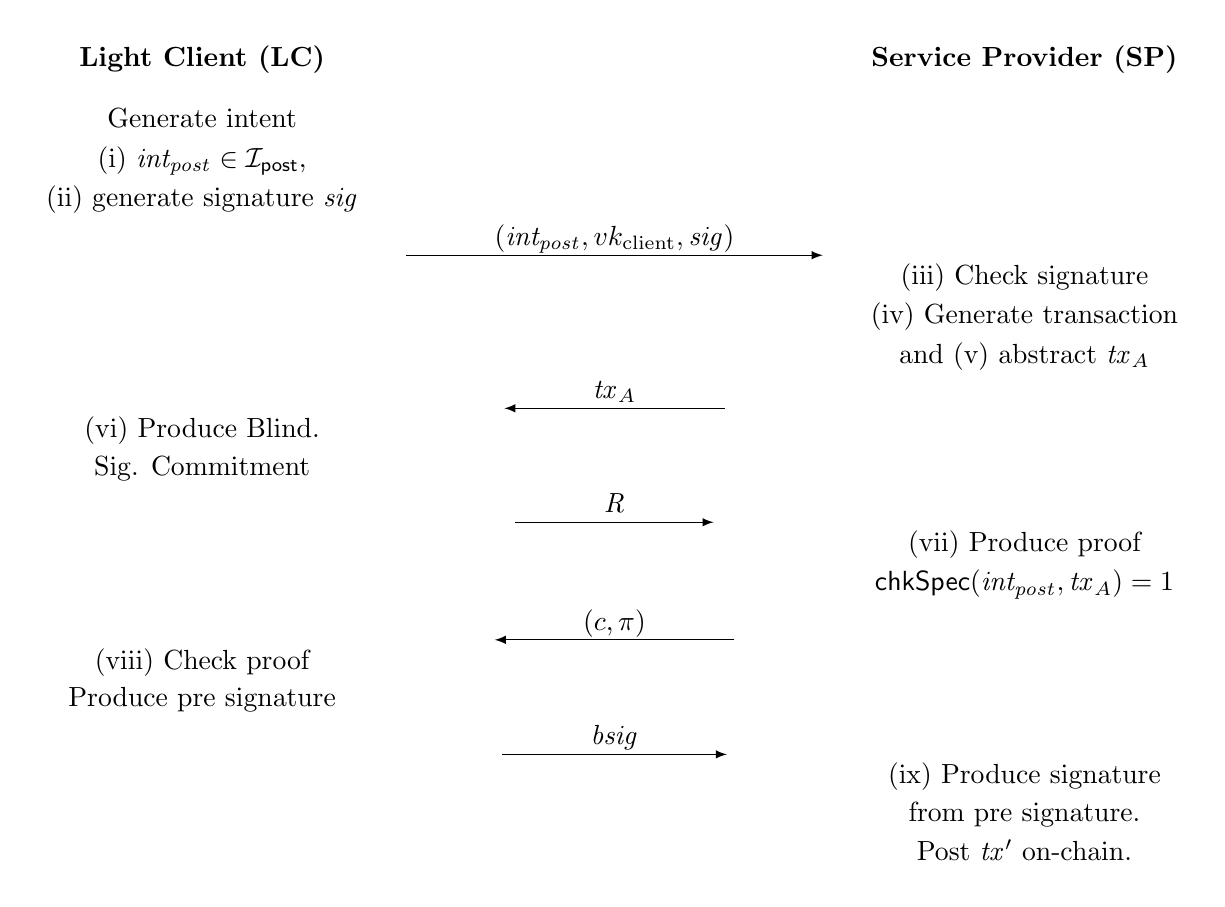
\begin{tikzpicture}
    \label{fig:protocol}
	\matrix (m)[matrix of nodes, column  sep=1.5cm,row  sep=7mm, nodes={draw=none, anchor=center,text depth=0pt} ]{
		\textbf{Light Client (LC)} & & \textbf{Service Provider (SP)}\\[-4mm]
		Generate intent & & \\[-7mm]
		(i) $\var{int_{post}} \in \mathcal{I}_\mathsf{post}$, & & \\[-7mm]
		(ii) generate signature $\var{sig}$  & & \\[-7mm]
		% and predicate $\fun{opt} : \TxAbs \to \B$\\
		&  $(\var{int_{post}}, vk_{\mathrm{client}}, \var{sig})$ & \\[-7mm] %\fun{opt}(\ ),\
		& & (iii) Check signature \\[-7mm]
		& & (iv) Generate transaction  \\[-7mm]
		& & and (v) abstract $\var{tx}_A$  \\[-7mm]
		& $\var{tx}_A$ & \\[-7mm]
		%\ h=\fun{txid}~\var{tx}
		% %& ZK.proof $p$ of $P (h,\  \var{tx}_A) = \true$ & \\
		(vi) Produce Blind.  \\[-7mm]
			Sig. Commitment \\[-7mm]
		% sign abstract transaction\\[-7mm]
		& $\var{R}$\\[-7mm]
		& & (vii) Produce proof   \\[-7mm]
		& & $\fun{chkSpec}(\var{int_{post}},\var{tx}_A) = 1$ \\[-7mm]
		& $(c,\pi)$ & \\[-7mm]
		% %& ZK.proof $p$ of $P (h,\  \var{tx}_A) = \true$ & \\
		(viii) Check proof \\[-7mm]
		Produce pre signature \\[-7mm]

		% sign abstract transaction\\[-7mm]
		& $\var{bsig}$\\[-7mm]
		& & (ix) Produce signature\\[-7mm]
		& & from pre signature.\\[-7mm]
		& & Post $\var{tx'}$ on-chain.\\
	};
	
	%\draw[shorten <=-1.5cm,shorten >=-1.5cm] (m-1-1.south east)--(m-1-1.south west);
	%\draw[shorten <=-1.5cm,shorten >=-1.5cm] (m-1-3.south east)--(m-1-3.south west);
	
	\draw[shorten <=-1cm,shorten >=-1cm,-latex] (m-5-2.south west)--(m-5-2.south east);
	\draw[shorten <=-1cm,shorten >=-1cm,-latex] (m-9-2.south east)--(m-9-2.south west);
	\draw[shorten <=-1cm,shorten >=-1cm,-latex] (m-12-2.south west)--(m-12-2.south east);
	\draw[shorten <=-1cm,shorten >=-1cm,-latex] (m-15-2.south east)--(m-15-2.south west);
	\draw[shorten <=-1cm,shorten >=-1cm,-latex] (m-18-2.south west)--(m-18-2.south east);

\end{tikzpicture}

\newpage


\begin{definition}[Correctness] A transaction building protocol is \textbf{correct} if for an honest light client, and service provider and any state $\LState$ and intent $\mathcal{I}_\mathsf{post}$ such that: if $\fun{mkToSpec}(\LState, \mathcal{I}_\mathsf{post}) \neq \bot$, then the protocol completes and the transaction $\Tx'$ produced by the SP is such that $\fun{\fun{checkTxL}~}(LState, \Tx')=1$. \end{definition}

\todobox{ Let ${\fun{checkTxL}~}(LState, \Tx)$  be shorthand for  $\fun{checkTx}~((\var{slot}, \var{fee}), \var{utxo},~\var{tx})$ }.


\begin{definition}[Safety] A transaction building protocol is \textbf{safe} if for an honest light client and any service provider SP we have that: if transaction $\Tx('$ is produced by the SP is such that  $\fun{\fun{checkTxL}~}(LState, \Tx')=1$  
%against the client's key (XXX note: maybe we can ommit this)
, then it must be that $\fun{chkSpec}(\mathcal{I}_\mathsf{post} , \Tx')=1$. \end{definition}

\begin{definition}[Private until posted] A transaction building protocol has the  \textbf{private until posted} property if a PPT adversarial client $C_\mathcal{A}$ cannot win the following experiment with probability significantly higher than $1\over 2$.

For an honest service provider SP and any client $C_\mathcal{A}$ we have that: client provides 2 states $\LState_0, \LState_1$ and one intent $\mathcal{I}_\mathsf{post}$ such that for $i=0,1$ it is $ \fun{mkToSpec}(\LState_i, \mathcal{I}_\mathsf{post}) \neq \bot$.  The experiment flips a coin $d$ and runs the protocol between SP and C* using state $\LState_d$. $C_\mathcal{A}$ outputs $d^*$. The adversarial client wins iff $d=d^*$. \end{definition}



\textbf{Single-SP vs Multi-SP Protocols. }
We describe a basic protocol in which a single LC queries a single SP for constructing a 
transaction matching LC's specification, and then eventually that transaction getting posted 
after all protocol steps are completed. We assume that all specification-meeting 
transactions are acceptable to the LC. However, we can also formulate a version of this 
protocol where the LC instead sends the specification to multiple SPs, selecting the best 
response, and engaging in the rest of the protocol only with that SP.

To do this, let $\fun{opt} : \TxAbs \to \Z$ be a function that rates abstract 
transactions to express LC's preferences. For example, the total amount of primary tokens 
spent by the transaction can be such a function :
$\fun{opt}~\var{tx} = \fun{coinValue}~(\sum_{o \in~\var{txd}.\fun{spentOuts}} \var{o}.\val)$. 
A transaction $\var{tx}$ is \emph{optimal} in a set $S \in \type{Set}~\TxAbs$ when 
 
 \[ \fun{opt}~\var{tx} = \fun{min}~\{~\fun{opt}~\var{tx'}~\vert~\var{tx'}~\in~S~\} \]

To get a multi-SP protocol, the first step of the single-SP protocol in Figure \ref{fig:protocol}
must be augmented, so that the pair $(\fun{opt}, \var{int_{post}}$ is sent to each SP instead of just
sending $\var{int_{post}}$. 
Upon receiving transactions $\var{tx}_{A,i}$, with $0\leq i < k$, from each of the $k$ SPs responding 
to LC's query, LC will engage in the rest of the protocol only with the sender of $\var{tx}_{A,i}$. 

 Note that the $\fun{opt}$ function and the specification serve different purposes in the protocol. 
 The specification is checked, and any response transaction that does not satisfy it is discarded.
 On the other hand, it is not required that a transaction be optimal across all possible 
 specification-satisfying transactions.  The kind of 
 sophisticated optimization (such as what is required, e.g., for optimized order-matching) would require 
 an entirely distinct set of tools for demonstrating the optimality result, such as ZK proofs about 
 the full blockchain state (rather than just the associated transaction), together with evidence that 
 the proof is about state that is \emph{sufficiently current} (see Section \ref{sec:stale-state}). 
 For example, a proof that 
 that there were no better offers for a specific token available on the ledger at the time the SP 
 produced a response to the LC. We do not assume that 
 either the SP or the LC are necessarily capable of performing or verifying (resp.) optimality according to the 
 function LC requested be optimized, but an LC is capable to comparing transactions using $\fun{opt}$.

 
 \section{Blind Signatures for Abstract Transactions}
 \label{sec:blind}
 In order to allow the LC to sign an abstract transaction artifacts we implement blind signatures on (partially) blinded transaction objects.
 At the minimum the SP hides the inputs to the transaction, i.e., the references to UTxO objects which are present in the ledger and required to cover the transaction.

 In Bitcoin, for example, UTxOs are captured in the ledger as follows:
 For Cardano, the structure looks as follows:

 \todobox{ Describe UTxO briefly for all chains we support?  }.


 The specific ledger implementation might require slight adaptations in terms of signature type and used hash functions---in this work, we give a very general construction that can be tailored to specific blockchains.

 Our construction is inspired by the predicate blind signature mechanism in~\cite{blindsigs}. 
 It realizes a concurrently secure blind and partially blind signing protocol resulting in  standard Schnorr signatures.
 The signature scheme builds upon the original protocol proposed in~\cite{10.1007/3-540-48071-4_7} with the addition of a commitment phase that binds the signer to her secrets (blinding value and message), preventing a forgery attack (described in~\cite{bibid}) and making the scheme unforgeable under concurrent sessions. 

 We describe how this protocol can be applied and simplified for abstract transaction signing.
 The proposed simplification is applicable in our setting due to the fact that our protocol does not rely on concurrent singing sessions.
 Furthermore, unlinkability of signatures and artifacts.
 Once the SP publishes final (unblinded) transactions on the chain, the LC can in theory download recent blocks and observe the transaction that was posted by the SP on behalf of the light client. If downloading is too resource-intensive, the LC might also consult an online block explorer for said purpose. As a consequence, abstract transactions, published transactions and signatures are assumed to be ``linkable'' and unlinkability provided by the signature scheme is redundant in our scenario.



 \todobox{ 
    \begin{itemize}
 \item Do we consider TLS connection between LC and SP? A network adversary could otherwise link/localize abstract transactions and transactions posted on the ledger. 
 \item specify the signing algorithm : $\fun{sign} : (\H, \privkey) \to \H$
 \item specify the function to make real sigs from blind sigs $\fun{mkRealSig} : (\pubkey \times \TxId \times \TxAbs \times \H) \to \H$
\item specify the blind signing algorithm $\fun{blindSign} : \H \times \TxAbs \times \privkey \to \H$
\end{itemize} }.

 





\section{Analysis}

\textbf{Asset and Non-Asset Compensation.} In our model, we have so far assumed that an SP performs its 
services in exchange for a fee. This fee may be either flat, or calculated on the basis of transaction size, 
or complexity of transaction specification, etc. - the details of this fee calculation are dependent on the 
specifics of the implementation of our protocol, the marketplace, and SPs preferences. 
The fee may also be specified in either an amount of primary asset tokens, 
or some other user-defined tokens. A fee requirement in user-defined tokens could be useful in the case 
of the SP service for LCs being associated with another type of service trading in such tokens, such as a 
videogame token marketplace. Yet another option for SPs is to request non-monetary compensation 
for their services, such as requiring engagement with a specific smart contract (i.e. SP does DApp fee 
sponsorship), voting for a specific update, 
delegating stake, etc. All these actions can be performed by the very transaction that SP constructed 
according to LC's specification. 


\section{Conclusion}



\begin{credits}
\subsubsection{\ackname} A bold run-in heading in small font size at the end of the paper is
used for general acknowledgments, for example: This study was funded
by X (grant number Y).

\subsubsection{\discintname}
It is now necessary to declare any competing interests or to specifically
state that the authors have no competing interests. Please place the
statement with a bold run-in heading in small font size beneath the
(optional) acknowledgments\footnote{If EquinOCS, our proceedings submission
system, is used, then the disclaimer can be provided directly in the system.},
for example: The authors have no competing interests to declare that are
relevant to the content of this article. Or: Author A has received research
grants from Company W. Author B has received a speaker honorarium from
Company X and owns stock in Company Y. Author C is a member of committee Z.
\end{credits}
%
% ---- Bibliography ----
%
% BibTeX users should specify bibliography style 'splncs04'.
% References will then be sorted and formatted in the correct style.
%
\bibliographystyle{splncs04}
\bibliography{lcbib}

\appendix
\section{Expanded Technical Backgroud}
\label{app:techbg}

\subsection{Discrete Log Groups}
\begin{definition} A group generator \GGen{} is a probabilistic polynomial time (p.p.t.) algorithm with input a security parameter $\lambda$ and outputs a group description $\G,g,q$ such that $\G$ is a group of prime order $q\approx 2^\lambda$ with generator $g$. We say that the discrete logarithm problem is hard w.r.t. \GGen{} if for all p.p.t $\A$ we have that

$$\Pr[(\G,g,q) \gets \GGen(1^\lambda); t\gets \Z_q; h\gets g^t: t=A(\G,g,q,h) ] \mbox{ is negligible in }\lambda.$$
\end{definition}

\subsection{ Public Key encryption and Schnorr Signatures}

A public key encryption scheme $\PKE$ comprises a set of polynomial time algorithms $\Keygen,\Enc,\Dec$ with the following syntax:
\begin{itemize}
\item $\Keygen(1^\lambda) \to (ek,dk)$. Creates a public/private keypair $ek,dk$. The encryption key $ek$ also defines the message space $\mathcal{M}$
\item $\Enc(ek,m;\rho) \to C$. Encrypts a message $m\in \mathcal{M}$ under the public encryption key $ek$. \item $\Dec(dk,C) \to m$. Decrypts a ciphertext $C$ using the private decryption key $dk$.
\end{itemize}

\begin{definition} A public key encryption scheme $\PKE$ is \emph{correct} if 
$$\Pr[ (ek,dk) \gets \PKE.\Keygen(1^\lambda); m\gets \mathcal{M}:\PKE.\Dec(sk,\PKE.\Enc(pk,m))=m ] =1.$$
\end{definition}

\begin{definition} A public key encryption scheme $\PKE$ is \emph{IND-CPA secure} if for all stateful p.p.t. adversaries \A, the difference
$$\left| \Pr[ (ek,dk) \gets \PKE.\Keygen(1^\lambda); (m_0,m_1)\gets A(ek);d\gets\{0,1\}; c^*\gets \PKE.\Enc(ek,m_d):A(c^*)=d ] - {1\over2} \right|$$
is negligible in $\lambda$.
\end{definition}

\begin{definition} The Schnorr digital signature scheme $\SDS$ is defined for a group generator $\GGen$ and a hash function generator $\HGen$ and operates as shown on Figure \ref{fig:schnorr}.\end{definition}


\begin{figure}[ht]
\fbox{%
  \begin{minipage}{0.95\textwidth}
    % Top minipage
    
    \begin{minipage}[t]{0.05\textwidth}
    \end{minipage}\hfill
    \begin{minipage}[t]{0.4\textwidth}
    
 \textbf{\uline{\bm{$\SDS.\Setup(1^\lambda)$}}}\\[0.5ex]
\mbox{$(\G,g,q) \gets \GGen(1^\lambda)$}\\
\mbox{$\hash\gets  \HGen(q)$}\\
\mbox{$sp \gets (\G,g,q,\hash)$}\\
$\textbf{return } sp\\$


      \textbf{\uline{\bm{$\SDS.\Sign (sk,m)$}}}\\[0.5ex]
\mbox{$(\G,g,q,\hash,x):\subseteq sk$}\\
\mbox{$r\gets \Z_q;\ R\gets g^x ;\ c\gets \hash(R,X,m)$}\\
\mbox{$s\gets (r+c\cdot x) \mod q$}\\
\mbox{$\textbf{return } \sigma \gets(R,s)$}\\
    \end{minipage}
    \hfill
    \begin{minipage}[t]{0.40\textwidth}
      \textbf{\uline{\bm{$\SDS.\Keygen (sp)$}}}\\[0.5ex]
\mbox{$(\G,g,q) :\subseteq sp$}\\
\mbox{$x\gets \Z_q;\ X\gets g^x$}\\
\mbox{$sk,vk \gets (par,x),(par,X)$}\\
$\textbf{return } (sk,vk)\\$\\


%\vspace{.5cm}
       \textbf{\uline{\bm{$\SDS.\Ver(vk,m,\sigma)$}}}\\[0.5ex]
$(\G,g,q,\hash,X):\subseteq vk$\\
$(R,s)\gets \sigma; c\gets \hash(R,X,m)$\\
$\textbf{return } (g^s=R\cdot X^c)$

    \end{minipage}
    \hfill
    \begin{minipage}[t]{0.1\textwidth}
    \end{minipage}

  \end{minipage}%
}

\caption{The  Schnorr signature scheme \SDS, with group and hash generators \GGen,   \HGen.}\label{fig:schnorr}

\end{figure}


\begin{definition} A digital signature scheme $\DS$ is \emph{correct} if 
$$\Pr[sp\gets \DS.\Setup(1^\lambda); (sk,vk) \gets \DS.\Keygen(sp); m\gets \mathcal{M_{S}}:\DS.\Ver(vk,m,Sign(sk,m))=1 ] =1.$$
\end{definition}

\begin{definition} A digital signature scheme $\DS$ is \emph{strongly existentially unforgeable against chosen message attacks}  (sEUF-CMA)  if for all p.p.t.  adversaries \A, we have  
$$\Pr[\textsf{sEUF-CMA}^{\A}_{\DS}(1^\lambda)] $$
is negligible in $\lambda$ where the game $\textsf{GsEUF-CMA}^{\A}_{\DS}$ is defined in Figure \ref{fig:seufcma}. \label{def:seufcma}
\end{definition}


\begin{figure}[ht]
\fbox{%
  \begin{minipage}{0.95\textwidth}
    % Top minipage
    
    \begin{minipage}[t]{0.05\textwidth}
    \end{minipage}\hfill
    \begin{minipage}[t]{0.5\textwidth}

      \textbf{\uline{\bm{$\textsf{GsEUF-CMA}^{\A}_{\DS}(1^\lambda)$}}}\\[0.5ex]
$sp \gets \DS.\Setup(1^\lambda); Q\gets \emptyset$\\
$(sk,vk)\gets \DS.\Keygen(sp)\\ (m^*,\sigma^*)\gets \A^{\textsf{OSig}}(vk)$\\
$\textbf{return } (m^*,\sigma^*)\neq Q \land \DS.\Ver(vk,m^*,\sigma^*)$
    \end{minipage}
    \hfill
    \begin{minipage}[t]{0.35\textwidth}
      \textbf{\uline{\bm{$\textsf{OSig}(m)$}}}\\[0.5ex]
$\sigma \gets \DS.\Sign(skk,m)$\\
$Q \gets Q\cup \{(m,s)\}$\\
$\textbf{return } \sigma$
    \end{minipage}
    \hfill
    \begin{minipage}[t]{0.1\textwidth}
    \end{minipage}

  \end{minipage}%
}

\caption{The security experiment $\textsf{sEUF-CMA}^{\A}_{\DS}$ and supporting oracle $\textsf{OSig}$.}\label{fig:seufcma}

\end{figure}

\subsection{Parametrized Non-Interactive Zero Knowledge Arguments}

Following \cite{blindsigs}, we define non-interactive zero knowledge arguments with regards to \emph parametrized polynomial relations $\mathcal{P}: \{0,1\}^* \times \{0,1\}^* \times \{0,1\}^*  \to \{0,1\}$, where the first argument represents a parameter set $par$ (e.g. a group description). Given a value of $par$, we say that $w$ is a witness for statement $\theta$ if $\mathcal{P}(par,\theta,w)=1$, i.e. $R=R_{par}(\theta,w):=\mathcal{P}(par,\theta,w)$ is an NP-relation, and $\Lang=\Lang_{par}$ is an NP-language. A NIZK for a relation  $\mathcal{P}$ operates as follows:
\begin{itemize}

\item $\mathsf{Rel}(1^\lambda) \to par$. Generates a parameter set $par$ that defines $R$ and $\Lang$.
\item $\Setup(par)\to (\crs,\tau)$. Generates a common reference string (CRS) and trapdoor $\tau$ used by the simulator. We assume the CRS contains a description of $R$.
\item $\Prove(\crs,\theta,w)\to \pi$. Given a CRS $\crs$, statement $\theta$ and witness $w$ for $\theta$, produces a proof $\pi$.  
\item $\Ver(\crs,\theta,\pi)\to \{0,1\}$. Given a CRS $\crs$, a statement $\theta$ and a  proof $\pi$ outputs 1 or 0, accepting or rejecting the proof.
\item $\SimProve(\crs,\theta,\tau)$. Given a CRS $\crs$, statement $\theta$ and traproor $\tau$ for $\crs$, produces a simulated proof $\pi$.
\end{itemize}


\begin{definition} A system $\NArgr$ is perfectly correct if for all unbounded adversaries $\A$ 
\begin{align*}
\Pr [par \gets \NArg.\mathsf{Rel}(1^\lambda);  (\crs,\tau)\gets \NArg.\Setup(par); (\theta,w) \gets A(crs):  \\
\neg{}R(\theta,w) \lor \NArg.\Ver(\crs,\theta,\NArg.\Prove(\crs,\theta,w))]=1 \\
\end{align*}
\end{definition}

\begin{definition} A system $\NArgr$ is adaptably computationally sound if for all p.p.t. adversaries $\A$ 
\begin{align*}
\Pr [par \gets \NArg.\mathsf{Rel}(1^\lambda);  (\crs,\tau)\gets \NArg.\Setup(par); (\theta,\pi) \gets A(crs):  \\
\neg{}L(\theta) \land {}\NArg.\Ver(\crs,\theta,\pi)] \mbox{ is negligible in $\lambda$.}
\end{align*}
\end{definition}

\begin{definition} A system $\NArgr$ is  computationally zero-knowledge if for all p.p.t. adversaries $\A$ 
\begin{align*}
|\Pr [par \gets \NArg.\mathsf{Rel}(1^\lambda);  (\crs,\tau)\gets \NArg.\Setup(par); d\gets\{0,1\}:  \\
d = A^{\mathsf{OProve}_d}(crs)] - {1\over2}|\mbox{ is negligible in $\lambda$, where}\\
\mathsf{OProve}_0(\theta,w):= \textbf{if } \neg R(\theta,w) \textbf{ return }\bot; \textbf{ return } \NArg.\Prove(\theta,w), \mbox{and} \\
\mathsf{OProve}_1(\theta,w):= \textbf{if } \neg R(\theta,w) \textbf{ return }\bot; \textbf{ return } \NArg.\SimProve(\theta,\tau).
  \end{align*}
\end{definition}

\newpage

\section{Additional Ledger Syntax}
\label{sec:appendix}

In Figure~\ref{fig:notation:nonstandard} we introduce the standard ledger syntax that we use throughout.

\begin{figure}[h!tb]
  \begin{align*}
    \H{}
    & =~\bigcup_{n=0}^{\infty}\{0,1\}^{8n}
    & \mbox{the type of bytestrings }
    \\
    (a, b)
    & :~\Interval{A}
    & \text{intervals over a totally-ordered set $A$}
    \\
    \var{Key} \mapsto \var{Value}
    & \subseteq \{~ k \mapsto v ~\mid~ k \in \var{Key},~v \in \var{Value}~ \}
    & \text{finite map with unique keys}
    \\
    [a1 ; ...; ak]
    & :~[C]
    & \text{finite list with terms of type $C$}
    \\
    h :: t
    & :~[C]
    & \text{list with head $h$ and tail $t$}
    \\
    x \cup \fun{nothing}
    & :~A^?
    & \text{maybe type over $A$}
    \\
    a ~\{ ~\fun{field} = ~x~\}
    & :~A
    & \text{record of type A with $\fun{field}$ changed to $x$}
  \end{align*}
  \caption{Notation}
  \label{fig:notation:nonstandard}
\end{figure}

Figure~\ref{fig:eutxo-types} lists the primitives and derived types
that comprise the foundations of the EUTxO model,
along with some ancillary definitions.
(Outputs normally refer to transaction IDs by hash,
but we simplify here for clarity.)

\begin{figure}[h!tb]

\textsc{Ledger primitives}
\begin{displaymath}
\begin{array}{rlll}
  \checkSig &:&
  \Tx \to \pubkey \to \H \to \B \\
  & &\mbox{\emph{checks that a given key signed a transaction}}
\end{array}
\end{displaymath}

\textsc{Helper functions}
    \begin{align*}
        &\fun{txid} : \Tx \to \TxId \\
        &\fun{txid}~\var{tx} = \fun{hash}~(\var{tx} ~\{ ~\fun{sigKeys} = ~\fun{dom}~(\var{tx} . \sigs) ,~\sigs = ~\emptyset~\})
        \nextdef
        &\fun{toMap} : \N \to [\TxOut] \to (\N \mapsto \TxOut) \\
        &\fun{toMap}(\_,~[~]) ~~~~~~~~~~~~~= [~] \\
        &\fun{toMap}(\var{ix},~u~::~\var{outs}) = \{~\var{ix}\mapsto u~\} \cup \fun{toMap}(\var{ix}+1,~\var{outs}) \\
        & \mbox{\emph{constructs a map from a list of outputs}}
        \nextdef
        &\fun{mkOuts} : \Tx \to \UTxO \\
        &\fun{mkOuts}(tx) = \{~(\var{tx},~\var{ix}) \mapsto o~ \mid~(\var{ix} \mapsto o)\in~\fun{toMap}(0,~\var{tx}.\outputs)~\} \\
        &\mbox{\emph{constructs a UTxO set from a list of outputs of a given transaction}}
        \nextdef
        &\fun{MOf} : \N \to \N \to (A \to \B) \to [A] \to \B \\
        &\fun{MOf}~k~m~f~[~] = m~\leq~k \\
        &\fun{MOf}~k~m~f~( h~ ::~ t) = \fun{if}~ (m~\leq~k)~\fun{then}~\true~\fun{else}~(\fun{MOf}~(k~+~a)~m~f~t) \\
        &~~\where~~a~=~\fun{if}~ (f~(h))~\fun{then}~1~\fun{else}~0 \\
        &\mbox{\emph{returns $\true$ if enough elements of a list satisfy given function}}
    \end{align*}
\caption{Primitives and basic types for the $\UTxO_{ma}$ model}
\label{fig:eutxo-types}
\end{figure}
\newpage 
\subsection{Transaction Validation Rules}

A transaction $\var{tx}$ is \emph{valid} if it follows the following rules. 

\label{sec:check-tx}


\begin{itemize}
    \item[(i)] \textbf{The transaction has at least one input:}
  \[
  \var{tx}.\inputs~\neq~\{\}
  \]
    \item[(ii)] \textbf{The current slot is within transaction validity interval:}
  \[
  \var{slot} \in \var{tx}.\fun{validityInterval}
  \]
    \item[(iii)] \textbf{All outputs have positive values:}
  \[
  \forall o \in \var{tx}.\outputs,~\var{o}.\val > \emptyset
  \]
    \item[(iv)] \textbf{All output references of transaction inputs exist in the UTxO:}
  \[
  \var{tx}.\inputs~ \subseteq~ \fun{dom}~\var{utxo}
  \]
    \item[(v)] \textbf{Value is preserved:}
  \[
  \var{tx}.\mint +
  \sum_{i \in~\var{tx}.\inputs,~(i~\mapsto~o) \in~\var{utxo}} \var{o}.\val =
  \sum_{o \in~\var{tx}.\outputs} \var{o}.\val ~+~\fun{toValue}~(\var{tx}.\fun{fee})
  \]
    \item[(vii)] \textbf{All inputs validate:}
  \[
  \forall~ i \in \var{tx}.\inputs,~i \mapsto (s, v) \in \var{utxo},~
     \applyScript{s}(\fun{dom}~(\var{tx}.\sigs),~\var{tx}.\validityInterval) = \true
  \]
    \item[(ix)] \textbf{All minting scripts validate:}
  \[
  \forall~ p\mapsto \_ \in \var{tx}.\mint,~ \applyScript{p} (\fun{dom}~(\var{tx}.\sigs),~\var{tx}.\validityInterval) = \true
  \]
    \item[(x)] \textbf{All signatures are correct:}
  \[
  \forall~ (pk \mapsto s) \in \var{tx}.\sigs,~ \checkSig (\var{tx}, pk, s) = \true
  \]
  \item[(i)] \textbf{The fee is sufficient:}
  \[
    \var{s}.\fun{minfee} \leq \var{tx}.\fun{fee} 
  \]
  \end{itemize}

\subsection{Script construction and Evaluation}
\label{sec:check-script}

In Figure \ref{fig:script} we present the constructors and evaluation rules for scripts, and in Figure \ref{fig:mktospec} we explain the transaction building function \fun{mkToSpec}.

\begin{figure}
    \textsc{Constructors of $\Script$} 
\begin{displaymath}
\begin{array}{rlll}
    \fun{RequireMOf}         &: \N \to [\Script] &\to~ \Script \\
    \fun{RequireSig}         &: \pubkey      &\to~ \Script \\
    \fun{RequireTimeStart}   &: \Slot        &\to~ \Script \\
    \fun{RequireTimeExpire}  &: \Slot        &\to~ \Script \\
\end{array}
\end{displaymath}
\nextdef
\textsc{Evaluation of $\Script$} 
\begin{displaymath}
\begin{array}{rlll}
  \applyScript{\_} &:& \Script \to ((\type{Set} \pubkey) \times (Slot \times Slot)) \to \B \\
  \applyScript{\fun{RequireMOf}~n~ls} (\var{khs}, (t1, t2)) &=&  \fun{MOf}~0~ n ~(\applyScript{\_}~(\var{khs}, (t1, t2))) ~ls \\
  \applyScript{\fun{RequireSig}~k} (\var{khs}, (t1, t2)) &=& k~\in~\var{khs} \\
  \applyScript{\fun{RequireTimeStart}~t1'} (\var{khs}, (t1, t2)) &=& t1'~\leq~t1 \\
  \applyScript{\fun{RequireTimeExpire}~t2'} (\var{khs}, (t1, t2)) &=& t2~\leq~t2' 
\end{array}
\end{displaymath}
\caption{$\Script$ constructors and evaluation}
\label{fig:script}
\end{figure}

\begin{figure}
      \textsc{Trivial transaction $\fun{initTx}_{a,mf}$} 
\begin{displaymath}
\begin{array}{rlll}
  \fun{initTx}_{a,mf}  &=& \{ ~\inputs = \emptyset,\\
  & &\ \outputs = [ (a , \fun{tip})],\\
  & &\ \fun{validityInterval} = [\fun{nothing} , \fun{nothing}],\\
  & &\ \mint = 0,\\
  & &\ \fun{fee} = mf \\
  & &\ \fun{aux} = []~\\
  & &\ \sigs = \emptyset~ \}
\end{array}
\end{displaymath}
\nextdef
\textsc{Input selection function} 
\begin{displaymath}
\begin{array}{rlll}
  \fun{mkIns}  &:& (\LState \times (\type{Set} \TxIn) \times \Value \times \Script) \to (\type{Set} \TxIn) \\
  \fun{mkIns} ~(l,~i,~v,~s) &=& \fun{if}~\neg~(v \leq 0) ~ \fun{then} \\
  & & ~~~~ \fun{if}~(v > 0)~\fun{then}~\\
  & & ~~~~ ~~~~\fun{mkIns}~(l~\setminus~(\{j \mapsto \_\}),~i \cup j,~v~-~(u(j) . \val) ,~s) \\
  & & ~~~~ \fun{else}~i\\
  & & \fun{else } \\
  & & ~~~~\fun{nothing} \\
  & & \fun{where}~\\
  & & ~~~j = \fun{pickInput}~l~s \\
  & & ~~~u = \fun{utxo}~l
\end{array}
\end{displaymath}
\nextdef
\textsc{Auxiliary $\fun{mkToSpec'}$ definition} 
\begin{displaymath}
\begin{array}{rlll}
\fun{mkToSpec'} &:& \LState \to \mathcal{I}_\mathsf{post} \to \Tx \to \Tx^? \\
\fun{mkToSpec'}~l~(\fun{MustMint}~v) (\var{tx}) &=&  \var{tx}~\{ \mint~=~v ~+~ \var{tx} . \mint , \fun{sigs} = tx.\fun{sigs} \cup \fun{getSigsVal}~v ,\\
& & ~~~~\fun{validityInterval} = \fun{restrictIntervalVal}~tx.\fun{validityInterval}~v\} \\
\fun{mkToSpec'}~l~(\fun{SpendFrom}~s) (\var{tx}) &=& \var{tx}~\{ \outputs~=~ \var{tx} . \inputs~\\
& & ~~~~\cup~\fun{newIns} , \fun{sigs} = tx.\fun{sigs} \cup \fun{getSigsUTxO}~\fun{newIns}~l ,\\ 
& & ~~~~ \fun{validityInterval} = \\ 
& &~~~~~~~~\fun{restrictIntervalUTxO}~tx.\fun{validityInterval}~\fun{newIns}~l\} \\
& & ~~~~\where \\
& & ~~~~\fun{newIns} = \fun{mkIns}~l~(\var{tx} . \inputs)~(\fun{produced} - \fun{consumed})~ s \\
\fun{mkToSpec'}~l~ (\fun{MaxInterval}~i) (\var{tx}) &=& \var{tx}~\{ \validityInterval~=~(l . \fun{slot}, \\
& & ~~~~\fun{min}~\{l . \fun{slot}~+~i , \var{tx} . \fun{validityInterval}_2)\} \}  \\
\fun{mkToSpec'}~l~ (\fun{PayTo}~(s, v)) (\var{tx}) &=& \var{tx}~\{ \outputs~=~ \var{tx} . \outputs~\cup~ (s, v) \}   \\
\fun{mkToSpec'}~l~ (\fun{ChangeTo}~s) (\var{tx}) &=& \fun{if}~ \fun{consumed} - \fun{produced} ~>~0 ~\\ 
& & ~~~~\fun{then}~ \var{tx}~\{ \outputs~=~ \var{tx} . \outputs~\\
& & ~~~~\cup~ \{(s,~ \fun{consumed} - \fun{produced})\} \} ~\fun{else}~\fun{nothing}   \\
\fun{mkToSpec'}~l~ (\fun{MaxFee}~f)~ (\var{tx}) &=&  \fun{if}~ \var{tx} . \fun{fee} \leq f~\\ 
& & ~~~~\fun{then}~\var{tx}~\fun{else}~\fun{nothing} \\
\fun{mkToSpec'}~l~ (\fun{AndExps}~[a1 ; a2 ; ... ; ak]) (\var{tx}) &=& \fun{mkToSpec'}~l~ak~(... ~(\fun{mkToSpec'}~l~a2~(\fun{mkToSpec'}~l~a1~\var{tx})))
\end{array}
\end{displaymath}
\nextdef 
\textsc{$\fun{mkToSpec}$ definition} 
\begin{displaymath}
\begin{array}{rlll}
\fun{mkToSpec} &:& (\LState \times \mathcal{I}_\mathsf{post}) \to \Tx^? \\
\fun{mkToSpec}~(l , i) &=& \fun{mkToSpec'}~l~i~\fun{initTx}_{a,mf}
\end{array}
\end{displaymath}
\caption{Building transactions according to the specific intent}
\label{fig:mktospec}
\end{figure}




\begin{figure}
\begin{displaymath}
\begin{array}{rlll}
  \fun{txi}_1 &=&(\outputs = \{~(s, t)~\},\\
  & &\ \fun{validityInterval} = [ \fun{slot}~l , (\fun{slot}~l) + j ],\\
  & &\ \mint = t,\\
  & &\ \fun{fee} = \fun{minfee}~l \\
  & &\ \fun{sigKeys} = \fun{getSignersVal}~t) 
  \nextdef 
  \fun{txi}_2 &=& (\outputs = \{ (\fun{RequireSig}~k2,~x)~,~(\fun{RequireSig}~k1~,\\& & ~(\fun{balance}~(\fun{mkIns}~l~\{\}~x~ (\fun{RequireSig}~k1))) - x) \} ,\\
  & &\ \fun{validityInterval}  = [~ \fun{nothing}~ , \fun{nothing}~],\\
  & &\ \mint  = \{~\} ,\\
  & &\ \fun{fee}  = \fun{minfee}~l \\
  & &\ \fun{sigKeys}  = \{~k1~\} )
\end{array}
\end{displaymath}
\caption{Abstract transaction examples}
\label{fig:txs}
\end{figure}

%

\end{document}
